\documentclass[10pt,fleqn]{article} % Derfault font size and left-justified equations
\usepackage[%
    pdftitle={Correction des SLCI : Correcteur PI},
    pdfauthor={Xavier Pessoles}]{hyperref}

\input{style/new_style}
\input{style/macros_SII}
\usepackage{multicol}
\usepackage{siunitx}
\usepackage{schemabloc}
%\usepackage{picins}
\fichetrue
%\fichefalse

\proftrue
\proffalse

\tdtrue
%\tdfalse

\courstrue
\coursfalse

\newif\ifnormal
\normaltrue
%\normalfalse

\newif\ifdifficile
\difficilefalse
%\difficiletrue

\newif\iftdifficile
\tdifficilefalse
%\tdifficiletrue

% -------------------------------------
% Déclaration des titres
% -------------------------------------

\def\classe{\textsf{PSI$\star$ -- MP}}
\def\xxnumpartie{Cycle 03}
\def\xxpartie{Concevoir la partie commande des systèmes asservis afin de valider leurs performances}


\def\xxnumchapitre{Chapitre 1 \vspace{.2cm}}
\def\xxchapitre{\hspace{.12cm} Correction des SLCI}

\def\discipline{Sciences \\Industrielles de \\ l'Ingénieur}
\def\xxtete{Sciences Industrielles de l'Ingénieur}

\def\xxposongletx{2}
\def\xxposonglettext{1.45}
\def\xxposonglety{19}%16

\def\xxonglet{\textsf{Cycle 03}}

\def\xxactivite{TD 99}
\def\xxauteur{\textsl{Xavier Pessoles}}


\def\xxtitreexo{Quille pendulaire \ifnormal $\star$ \else \fi \iftdifficile $\star\star\star$ \else \fi }
\def\xxsourceexo{\hspace{.2cm} \footnotesize{Concours Commun Mines Ponts 2014}}

\def\xxcompetences{%
\textsl{%
\textbf{Savoirs et compétences :}\\
}}

\def\xxfigures{
\includegraphics[width=.75\textwidth]{images/fig_00}
}%figues de la page de garde
\def\xxpied{%
Cycle 03 -- Concevoir la commande des SLCI\\% afin de valider leurs performances.\\
Chapitre 1 -- \xxactivite%
}


\setcounter{secnumdepth}{5}
%---------------------------------------------------------------------------


\begin{document}
%\chapterimage{png/Fond_Cin}
\input{style/new_pagegarde}
\vspace{4.5cm}
\pagestyle{fancy}
\thispagestyle{plain}


\def\columnseprulecolor{\color{ocre}}
\setlength{\columnseprule}{0.4pt} 

\ifprof
%\begin{multicols}{2}
\else
\begin{multicols}{2}
\fi


\section*{Mise en situation}
\ifprof
\else

Les actions de l'air et de l'eau permettent au voilier d'avancer mais provoquent aussi son inclinaison autour de l'axe longitudinal $\vect{z_N}$. C’est le phénomène de gîte. Pour contrebalancer ce mouvement et éviter que le voilier ne se couche sur l’eau, la quille joue le rôle de contrepoids. 


%\begin{center}
%\includegraphics[width=.8\linewidth]{images/fig_01}
%%\textit{}
%\end{center}

Une évolution récente des voiliers de course océanique a été de les doter d’une quille pendulaire. Cette quille est en liaison pivot d’axe $\left(O,\vect{z}_N \right)$ avec la coque du navire et peut être orientée d’un côté ou de l’autre du navire. Une fois l’orientation désirée obtenue, tout mouvement dans la liaison pivot est supprimé par le blocage en rotation de celle-ci. 

\begin{center}
\includegraphics[width=.6\linewidth]{images/fig_03}

\textit{Modèle volumique 3D}
\end{center}



Afin de garantir sa répétabilité, la mise en position angulaire de la quille fait l’objet d’un contrôle par une boucle d’asservissement, dont le cahier des charges est donné ci-dessous.


\begin{center}
\begin{tabular}{|p{.7\linewidth}|c|}
\hline
Exigences & Niveau \\
\hline\hline
Stabilité : & \\
C11 : Marge de gain & \SI{10}{dB} \\
C12 : Dépassement vis-à-vis d'une entrée en échelon & Aucun \\
\hline
Rapidité :  & \\
C21 : Temps de réponse à 5\, \% & \SI{4}{s} maxi  \\
C22 : Vitesse angulaire de rotation de la quille & $8\degres/\text{s}$  maxi\\
\hline
Précision & \\
 C3 : Erreur statique vis-à-vis d'une entrée en échelon & Nulle \\
\hline
\end{tabular}
\end{center}


\subsection*{Modélisation du vérin}

La quille est manoeuvrée par deux vérins hydrauliques. Chacun d’eux est piloté par une servovalve de débit. Ce composant délivre un débit $q(t)$ proportionnel à sa tension de commande $v(t)$. Lors d’une manoeuvre de quille un seul de ces vérins est moteur et alimenté en pression via sa servovalve. L’autre est laissé dans une configuration où sa tige est libre de tout mouvement. Le déplacement terminé, la quille est verrouillée en position par un système de blocage non étudié dans ce sujet qui interdit toute circulation de fluide entre vérins et servovalves. L’angle de rotation de la quille par rapport au bâti est mesuré par un capteur potentiométrique.


Lors d’un déplacement de la quille, les mouvements d’oscillation du cylindre de vérin par rapport à la coque étant de faible amplitude et s’effectuant à de faibles vitesses, on se place dans une situation où le corps de vérin est considéré comme fixe. La tige est alors considérée en mouvement de translation galiléen.
On considère également que les mouvements étudiés sont de petits mouvements autour d’une position moyenne et que l’hypothèse des conditions initiales nulles est valide. Dans ces conditions, le comportement du vérin est défini par le modèle continu ci-dessous.

\footnotesize
\begin{center}
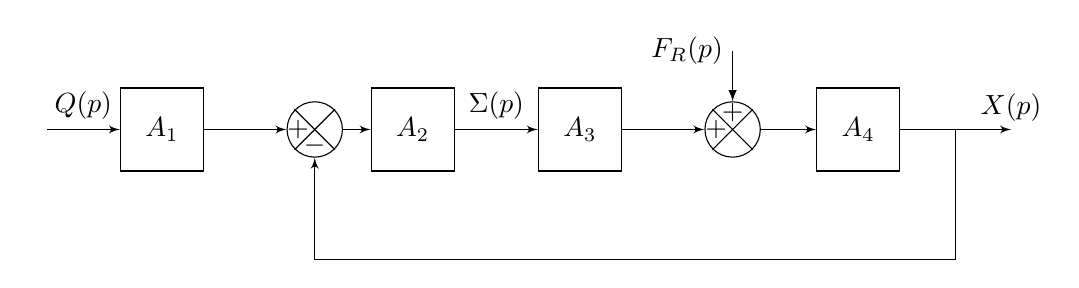
\begin{tikzpicture}
\sbEntree{E}

\sbBloc[3]{b0}{$A_1$}{E}
    \sbRelier[$Q(p)$]{E}{b0}


\sbComp{c1}{b0}
    \sbRelier{b0}{c1}

\sbBloc[1]{b1}{$A_2$}{c1}
    \sbRelier{c1}{b1}
    
\sbBloc[3]{b11}{$A_3$}{b1}
    \sbRelier[$\Sigma(p)$]{b1}{b11}


\sbSumh{c2}{b11}
    \sbRelier{b11}{c2}

\sbBloc{b2}{$A_4$}{c2}
    \sbRelier{c2}{b2}
    

\sbSortie[4]{S}{b2}
    \sbRelier{b2}{S}
    \sbNomLien[0.8]{S}{$X(p)$}
  
\sbRenvoi{b2-S}{c1}{}

\draw [latex-] (c2) --++ (0,1) node[left] {$F_R(p)$};

\end{tikzpicture}
\end{center}
\normalsize

On a : 
\begin{itemize}
\item $q(t)=S\dfrac{\dd x(t)}{ \dd t}+\dfrac{V}{2B}\dfrac{\dd \sigma(t)}{\dd t}$ (a);
\item $M\dfrac{\dd^2 x(t)}{\dd t^2} = S \sigma(t) - kx(t)-\lambda \dfrac{\dd x(t)}{\dd t} - f_R(t)$ (b).
\end{itemize}

On a :

\section{Titre 1}
\subsection{Titre 1.1}
\begin{corrige}
\end{corrige}

\subsection{Titre 1.2}
\begin{obj}
\end{obj}
\subsubsection{Titre 1.2.1}
\begin{warn}
\end{warn}
\subsubsection{Titre 1.2.2}
\section{Titre 2}
\begin{demo}
\end{demo}

\begin{exemple}

\end{exemple}

\begin{methode}
\end{methode}

\begin{resultat}
\end{resultat}

\begin{defi}
\end{defi}

\end{multicols}


\end{document}

\subparagraph{}\textit{}
\ifprof
\begin{corrige}
\end{corrige}
\else
\fi

\begin{center}
\includegraphics[width=\linewidth]{images/fig_04}
%\textit{}
\end{center}

